\chapter{Design}
\label{chap:design}

\section{Architecture Model}

The design is compatible with the C4 model, which describes software architecture through hierarchical abstractions: software systems, containers, components, and code \cite{c4-model}. For this project, one software system contains a mobile and web application container, local persistence, and external model and ingest systems. Inside the app container, responsibilities are distributed across screens, providers, services, repositories, and API route handlers.

Figure~\ref{fig:component-diagram} shows this separation explicitly, including how user-facing screens delegate business behavior to services and repositories.

\begin{figure}[H]
  \centering
  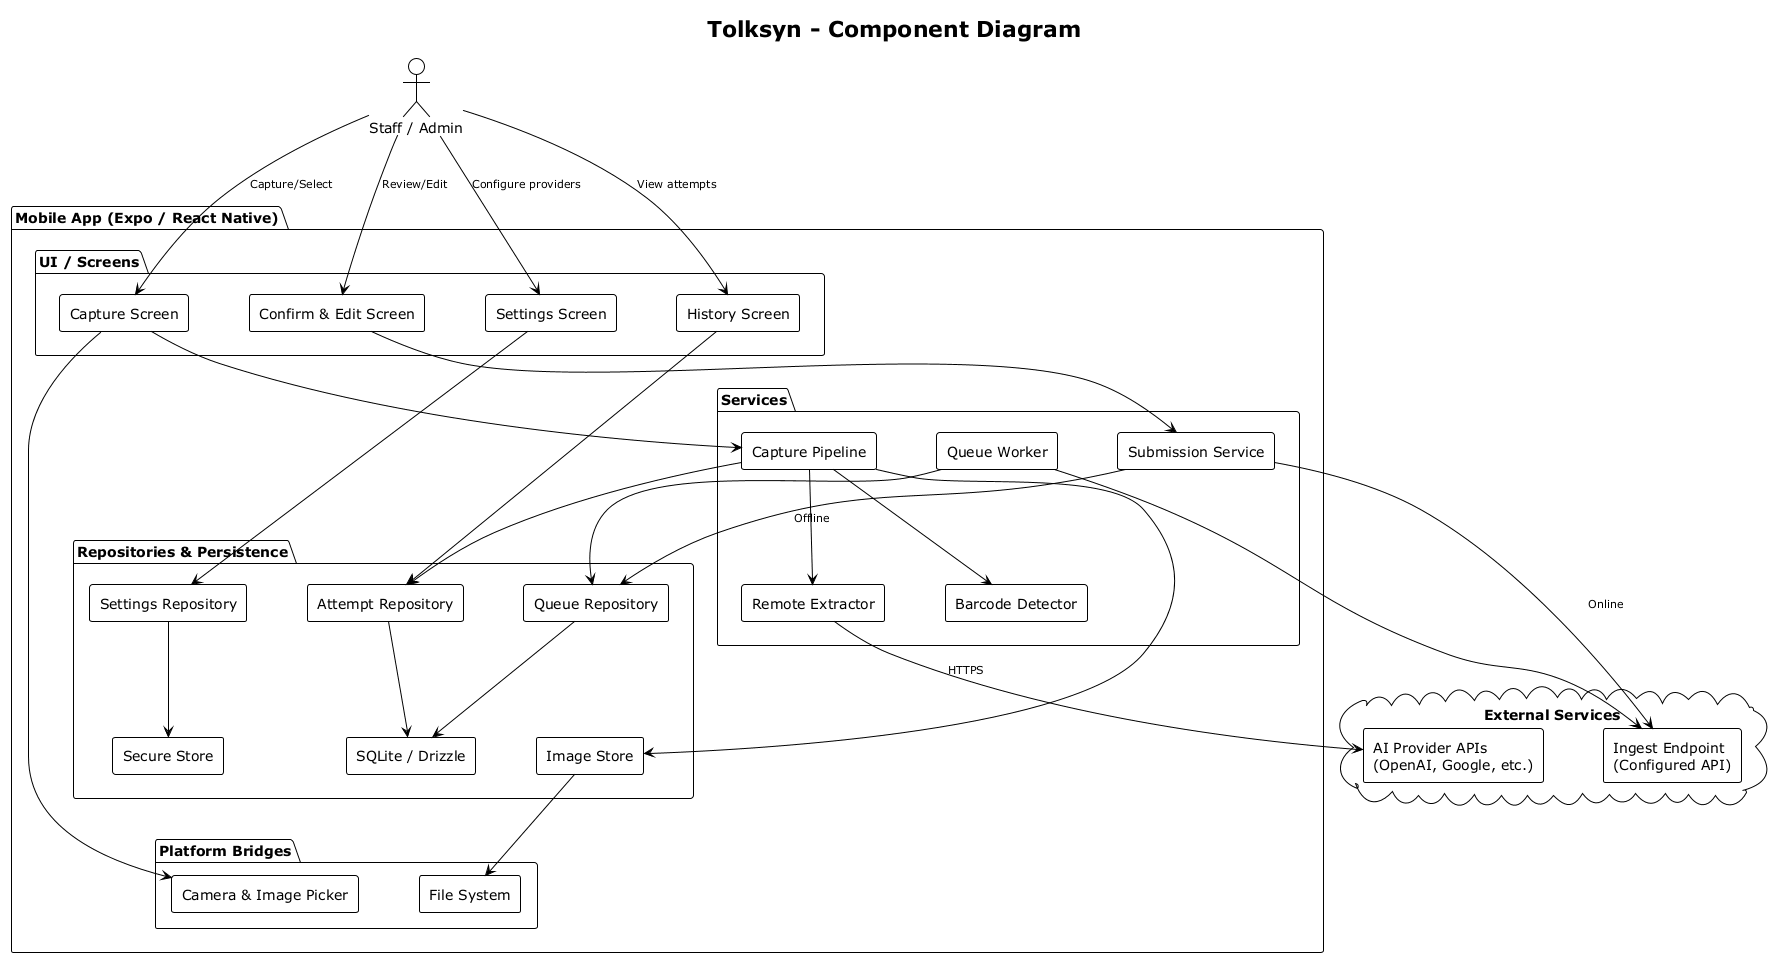
\includegraphics[width=0.95\textwidth,max height=0.58\textheight,keepaspectratio]{artifacts/component-diagram.png}
  \caption{Component diagram: routes and screens express user flow, while providers, services, repositories, and API modules handle runtime composition, persistence, extraction, and submission.}
  \label{fig:component-diagram}
\end{figure}

Table~\ref{tab:component-responsibility} complements this by listing the component boundaries and separation rationale.

\begin{table}[H]
\centering
\begin{tabularx}{\textwidth}{>{\raggedright\arraybackslash}p{0.25\textwidth}XX}
\toprule
Component & Responsibility & Reason for separation \\
\midrule
Screen modules & Render workflow state and collect user decisions & Keeps route files thin and UI focused. \\
App runtime provider & Composes database, settings, services, and queue worker & Central dependency wiring avoids scattered setup. \\
Capture pipeline & Coordinates image storage, barcode, extraction, merge, and persistence & Makes the end-to-end workflow testable. \\
Repositories & Read and write attempts, queue items, and settings & Isolates persistence details from business logic. \\
API routes & Proxy provider and web-search calls for web runtime & Keeps browser constraints away from screens. \\
\bottomrule
\end{tabularx}
\caption{Component responsibility model.}
\label{tab:component-responsibility}
\end{table}

\section{Capture-to-Ingest Pipeline}

The core pipeline distinguishes two evidence sources from the start: local barcode detection and provider-based vision-language extraction. Barcode detection is local and independent from provider routing, while the model provider only handles image-to-JSON extraction. The central design is deterministic: preprocess, run both extraction paths in parallel, merge, validate, confirm, then send.

Figure~\ref{fig:pipeline} visualizes this end-to-end loop.

\begin{figure}[H]
  \centering
  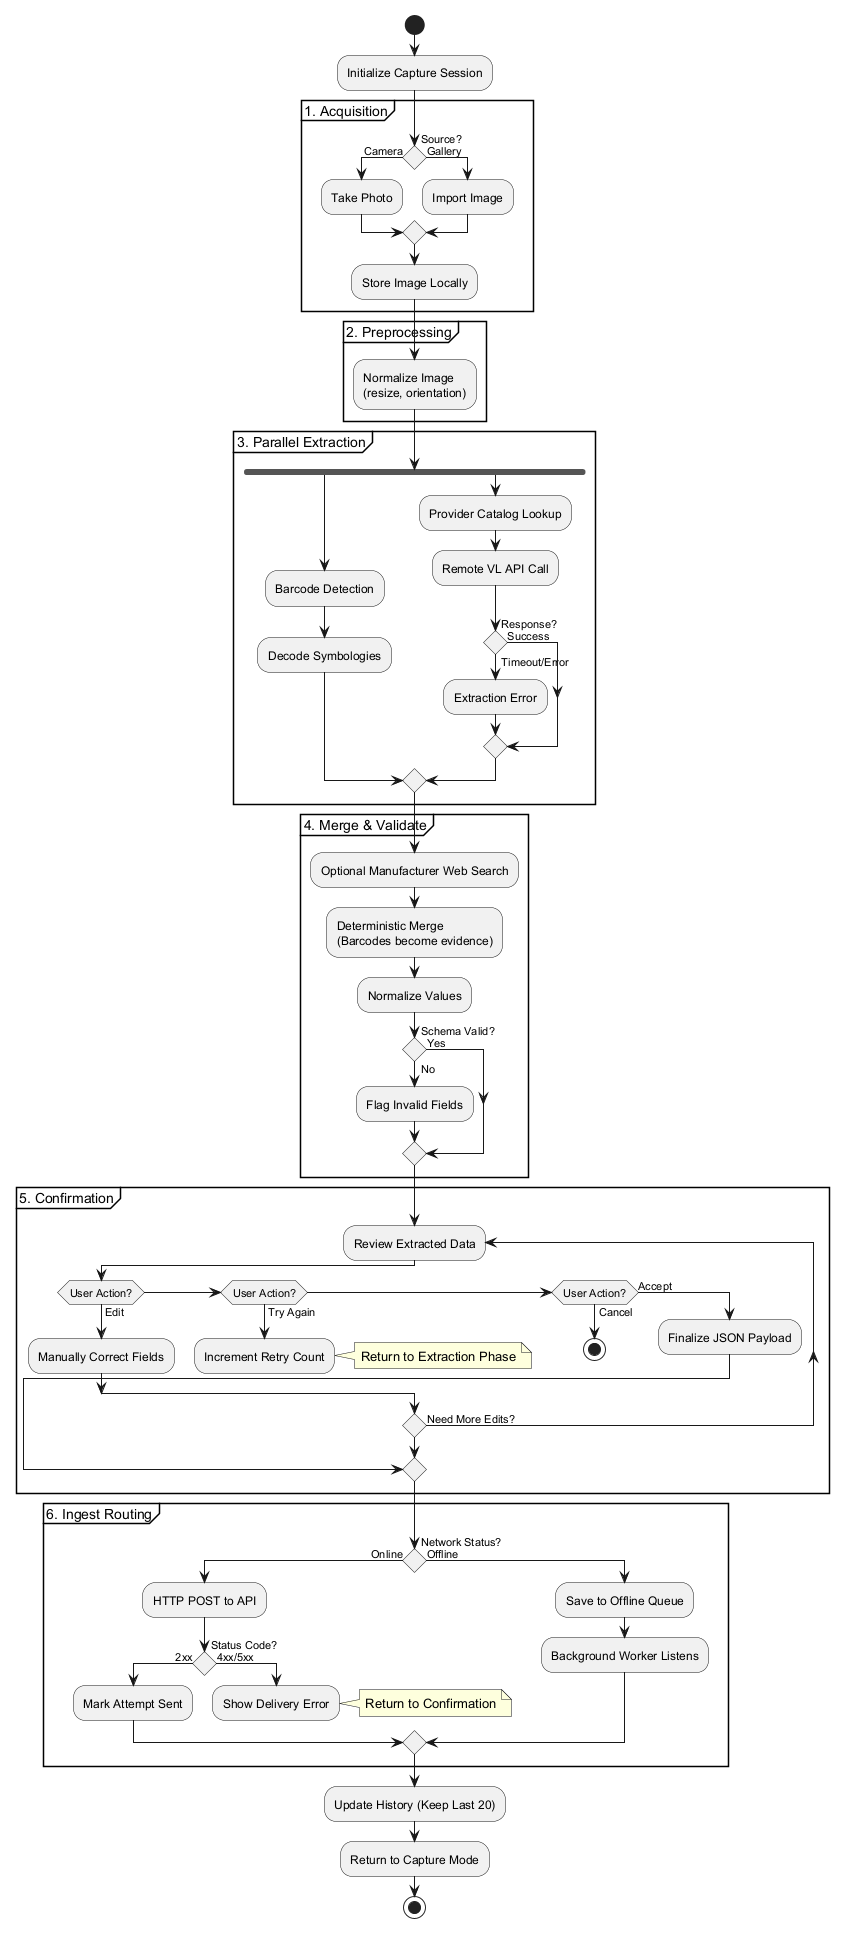
\includegraphics[height=0.78\textheight,max width=0.95\textwidth,keepaspectratio]{artifacts/app-pipeline-activity.png}
  \caption{Activity diagram: image storage, barcode detection, extraction, merge, validation, review, submission, and queueing are represented as one end-to-end capture-to-ingest workflow.}
  \label{fig:pipeline}
\end{figure}

The flow is:
\begin{itemize}
  \item user captures or imports an image,
  \item ImageStore normalizes the image and creates a thumbnail,
  \item AttemptRepository creates an attempt snapshot,
  \item barcode detection and remote extraction run in parallel,
  \item optional web-search enrichment adds manufacturer evidence,
  \item merge and validation produce a draft structured JSON object,
  \item the user edits and accepts the payload,
  \item SubmissionService sends immediately or queues with an idempotency key.
\end{itemize}

\section{Data Model}

Each capture is represented as an attempt. Attempt records store image URIs, timestamps, status, draft JSON, accepted revision, extraction result, and error code. Queue items store serialized payloads, retry state, idempotency keys, and attempt revision. Settings store non-secret configuration, while provider and ingest secrets are routed through the secret store abstraction. Figure~\ref{fig:persistence-model} shows the local data model used for this state.

\begin{figure}[H]
  \centering
  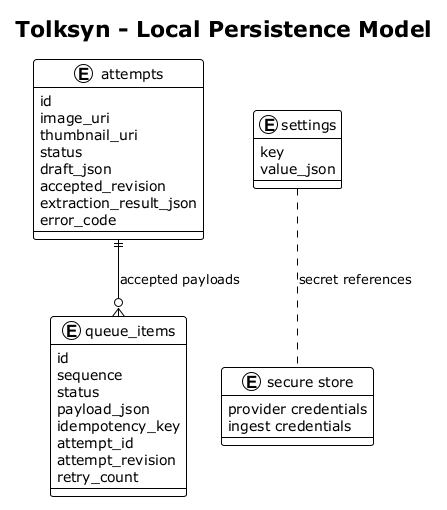
\includegraphics[width=0.88\textwidth,max height=0.62\textheight,keepaspectratio]{artifacts/local-persistence-model.png}
  \caption{Data model diagram: attempts, queue items, settings, and secure secret storage form the local state needed for review and replay.}
  \label{fig:persistence-model}
\end{figure}

\section{User Interface Design}

The user interface is organized around four main surfaces: Capture, Confirm and Edit, History, and Settings. Capture is optimized for fast repeated scans. Confirm and Edit gives the operator visibility into structured fields, barcode evidence, and diagnostics. History provides traceability for recent attempts. Settings makes the app portable across providers and ingest environments.

Figure~\ref{fig:ui-flow} summarizes the runtime navigation, while the design-stage Figma artifact is included as appendix evidence in Table~\ref{tab:evidence-artifacts}.

\begin{figure}[H]
  \centering
  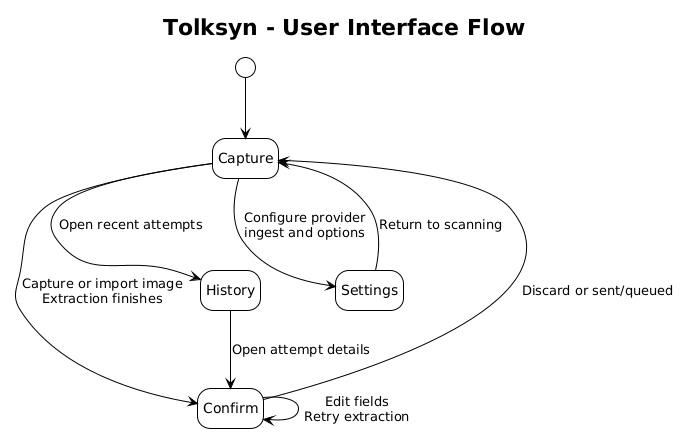
\includegraphics[width=0.92\textwidth,max height=0.58\textheight,keepaspectratio]{artifacts/ui-flow.png}
  \caption{User-flow diagram: navigation across Capture, Confirm and Edit, History, and Settings.}
  \label{fig:ui-flow}
\end{figure}

\section{Security and Privacy Design}

The project requires secrets to be stored securely, HTTPS for remote calls, no telemetry by default, and diagnostics with secret redaction. Expo SecureStore encrypts and securely stores key-value pairs locally on Android and iOS, using Android Keystore-backed encrypted SharedPreferences and iOS Keychain services \cite{expo-securestore}. The production deployment should enforce HTTPS ingest endpoints and ensure that web deployments apply the same secret-handling policy appropriate to the browser environment.

\section{State Model}

Attempt state is explicit. A typical attempt moves from \emph{captured} to \emph{ready for review}, then to \emph{sent} or \emph{queued} after user acceptance. Failure states distinguish \emph{extraction failed} from \emph{send failed}. Attempts that are sent, queued, or failed remain visible until retention pruning, while user-discarded and aborted partial attempts are removed from local history. This state model supports retry, history display, and queue replay without relying on transient UI state.

Figure~\ref{fig:state-model} shows the explicit transitions that support retry and queue replay behavior.

\begin{figure}[H]
  \centering
  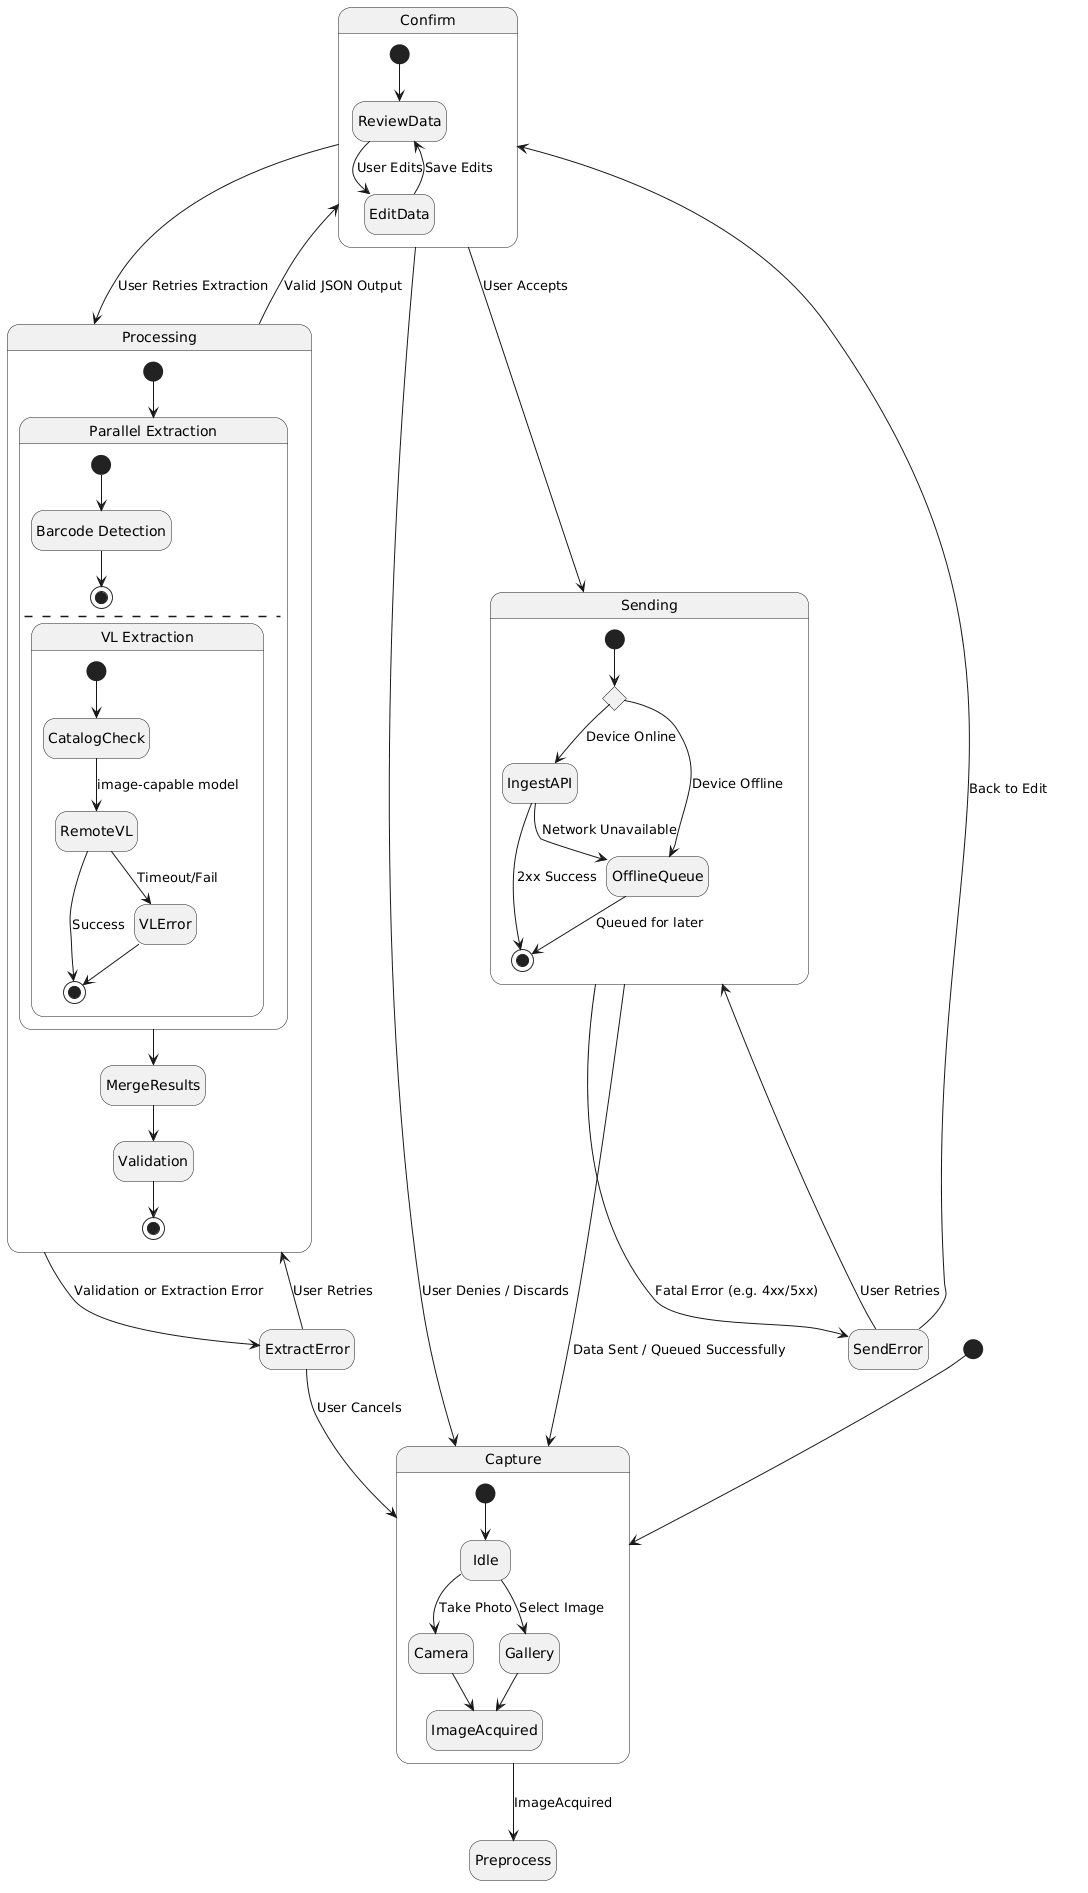
\includegraphics[height=0.78\textheight,max width=0.95\textwidth,keepaspectratio]{artifacts/app-state-machine.png}
  \caption{State-machine diagram: explicit attempt statuses make retry, history, discard, queueing, and delivery behavior visible.}
  \label{fig:state-model}
\end{figure}
